 \subsection{Software agents are now drivers...}
The NHSTA describes Level 4 autonomous vehicles as designed:
\begin{displayquote}
	\emph{To perform all safety-critical driving functions and monitor roadway conditions for an entire trip. Such a design anticipates that the driver will provide destination or navigation input, but is not expected to be available for control at any time during the trip. This includes both occupied and unoccupied vehicles. By design, safe operation rests solely on the automated vehicle system.} 
\end{displayquote}

In a letter to \emph{Google Inc.} regarding their Level 4 autonomous vehicles, the NHSTA states:
\begin{displayquote}
	\emph{Once the AV is determined to be the driver for purposes of a particular standard or test, the next question whether and how Google could certify that the SDS meets a standard developed and designed to apply to a human driver. In order for the NHSTA to interpret a standard as allowing certification of compliance by a vehicle manufacturer, NHSTA must first have a test procedure or other means of verifying such compliance.}
\end{displayquote}

Given this interpretation of the latest AV technology, and the ever-growing gap between the capabilities of current testing frameworks and regulations several pressing questions \emph{must} be answered:
\begin{itemize}
	\item The NHTSA states AV software is considered a driver. How does one bound the risk posed to society by an autonomous software agent?
	\item A driver's license is a set of tests, we attempt to generalize human behavior based on tests. AV's don't necessarily fail in predictable ways. Tests cover an infinitesimal portion of the state space. How do we gain confidence that algorithms are sound, free of bugs, or even ethical?
\end{itemize}

Our perspective encompasses an integrated approach that captures the manifestation of errors in the physical world. At its heart is the use of formal models of system and precise mathematical specifications of desired behavior. Specifically in APEX, we are interested in developing the appropriate formal models, a set of specifications, and a battery of testable scenarios. As part of this work we must investigate how such methods scale, or fail to scale, and provide new solutions and interfaces to the underlying tools. 
 
 \subsection{How do you give a self-driving car a driver's license?}
 Each year there are an average of 1.24 million traffic fatalities around the world \cite{Waldrop2015}. Estimates indicate that more than 90 percent of all accidents are due to driver error \cite{Waldrop2015}. Competent autonomous vehicles (AVs) could drastically reduce the occurrence of such incidents, but a major question first needs be answered:
 how can we judge when an AV is ready to graduate from research laboratories to public roads?
 One thing is clear: the public will want significant evidence that AVs are indeed safe \cite{weld1994first}. 
 This raises significant ethical and legal questions about how the AV should behave, and technical questions about how to \emph{verify} that it will always behave the way its designers intended.
 
 Prototype AVs have driven millions of miles and are even being approved for \emph{testing} on public roads in some states \cite{Iozzio2014}; however, manufacturers cannot \emph{verify} (i.e., guarantee) the safety of even the simplest of scenarios in the presence of other dynamic traffic participants. 
 Compounding the difficultly of vehicle certification, vehicle manufacturers such as Tesla are transitioning to frequent over-the-air software updates. Such practice eschews conventional vehicle development technique and greatly increases pressure on developers to deliver correct software at a rapid pace. 
 
 The net result is a wide gap between current regulations and our technological capabilities. 
 Human drivers are not `certified' to act safely in all situations, in fact, we know they don't; however, they assume liability for their actions.
 Who is liable for the behavior of an AV? The manufacturer or the vehicle owner?
 Currently, it appears that manufacturers will take one of two approaches: (1) assume liability for the actions of the vehicle and self-insure \cite{volvo15Liability} or (2) force the human occupants of an AV to make all critical decisions and shift liability to the pilot \cite{maurer2015autonomes}. In either case, even if AVs reduce accidents by 99 percent, it is likely that the 1 percent of remaining accidents will invariably spawn a myriad of legal actions against \emph{both} manufacturers \cite{russell2015research} and vehicle owners.   
 If the legal question is not answered, these risks could stifle the development of the AV market.
 
 Thus, regardless of where legal liability falls it is clear that we first need new, practical methods for verification and validation of the decision engines of each AV.
 Furthermore, verification must be automatic, exhaustive, and expedient for clearly defined scenarios. 
 Secondly, ethical considerations still underlie both the design and verification of AVs: how does the safety of the car's passengers weigh against that of people in its environment? 
 Whose morals are embedded in the decision engines of an AV?
 
 \subsection{New and Old Challenges}
 
 Some of the problems facing would-be AV manufacturers in 2016 are very similar to those outlined by the teams in the DARPA Urban Challenge \cite{buehler2009darpa}. One problem highlighted by the first ever crash between AVs at the Urban Challenge \cite{fletcher2008cornell} is that there are no known \quotes{formal methods that would allow definitive statements about the completeness or correctness of a vehicle interacting with a static environment, much less a dynamic one} \cite{urmson2008autonomous}.  Today one must still consider the massive configuration space of each individual snapshot of the day-to-day life of an AV if verification is to be attempted. For example, in order to test the interaction between two 7 DOF AVs requires $10^{14}$ simulations for only 10 samples from each state. If each test takes 10 seconds, the resulting set of simulations will take \emph{30 million years} to complete. Furthermore, within a given scenario, errors in localization, sensing, and actuation imply we never know the state of the world exactly. Small state estimation errors can befuddle motion planning algorithms and mean a difference between collision and safety in tight spots. As many teams in the Urban Challenge noted, a means of verifying the safety of autonomous driving is paramount to putting self-driving cars in the hands of the public \cite{urmson2008autonomous}. 
 
 In contrast to the Urban Challenge in 2007, in which only 6 teams out of an original 89 applicants were able to finish, many research labs find themselves in the position of being able to construct a convincing AV in a matter of months; such a vehicle might be relatively competent in 75 percent of the situations it faces, but the long tail of special cases beckons. In fact Sebastian Thrun, a veteran of Google's Self Driving Car project and the Urban Challenge, notes that \emph{there were many more of unusual situations than we believed in the beginning}. One possible solution to handling rare events and scenarios is to record such occurrences using consumer vehicles driving in real traffic; with each new scenario existing behavioral planners can be adjusted via a reinforcement learning scheme \cite{wei2013autonomous, Silver_2010, Waldrop2015}. Just as in the more vanilla scenarios, timely updates to controllers provided on the basis of a single example will need to be verified offline, before shipping, and without the thousands of miles of testing necessary for a typical safety feature. 
 
 \begin{figure}
 	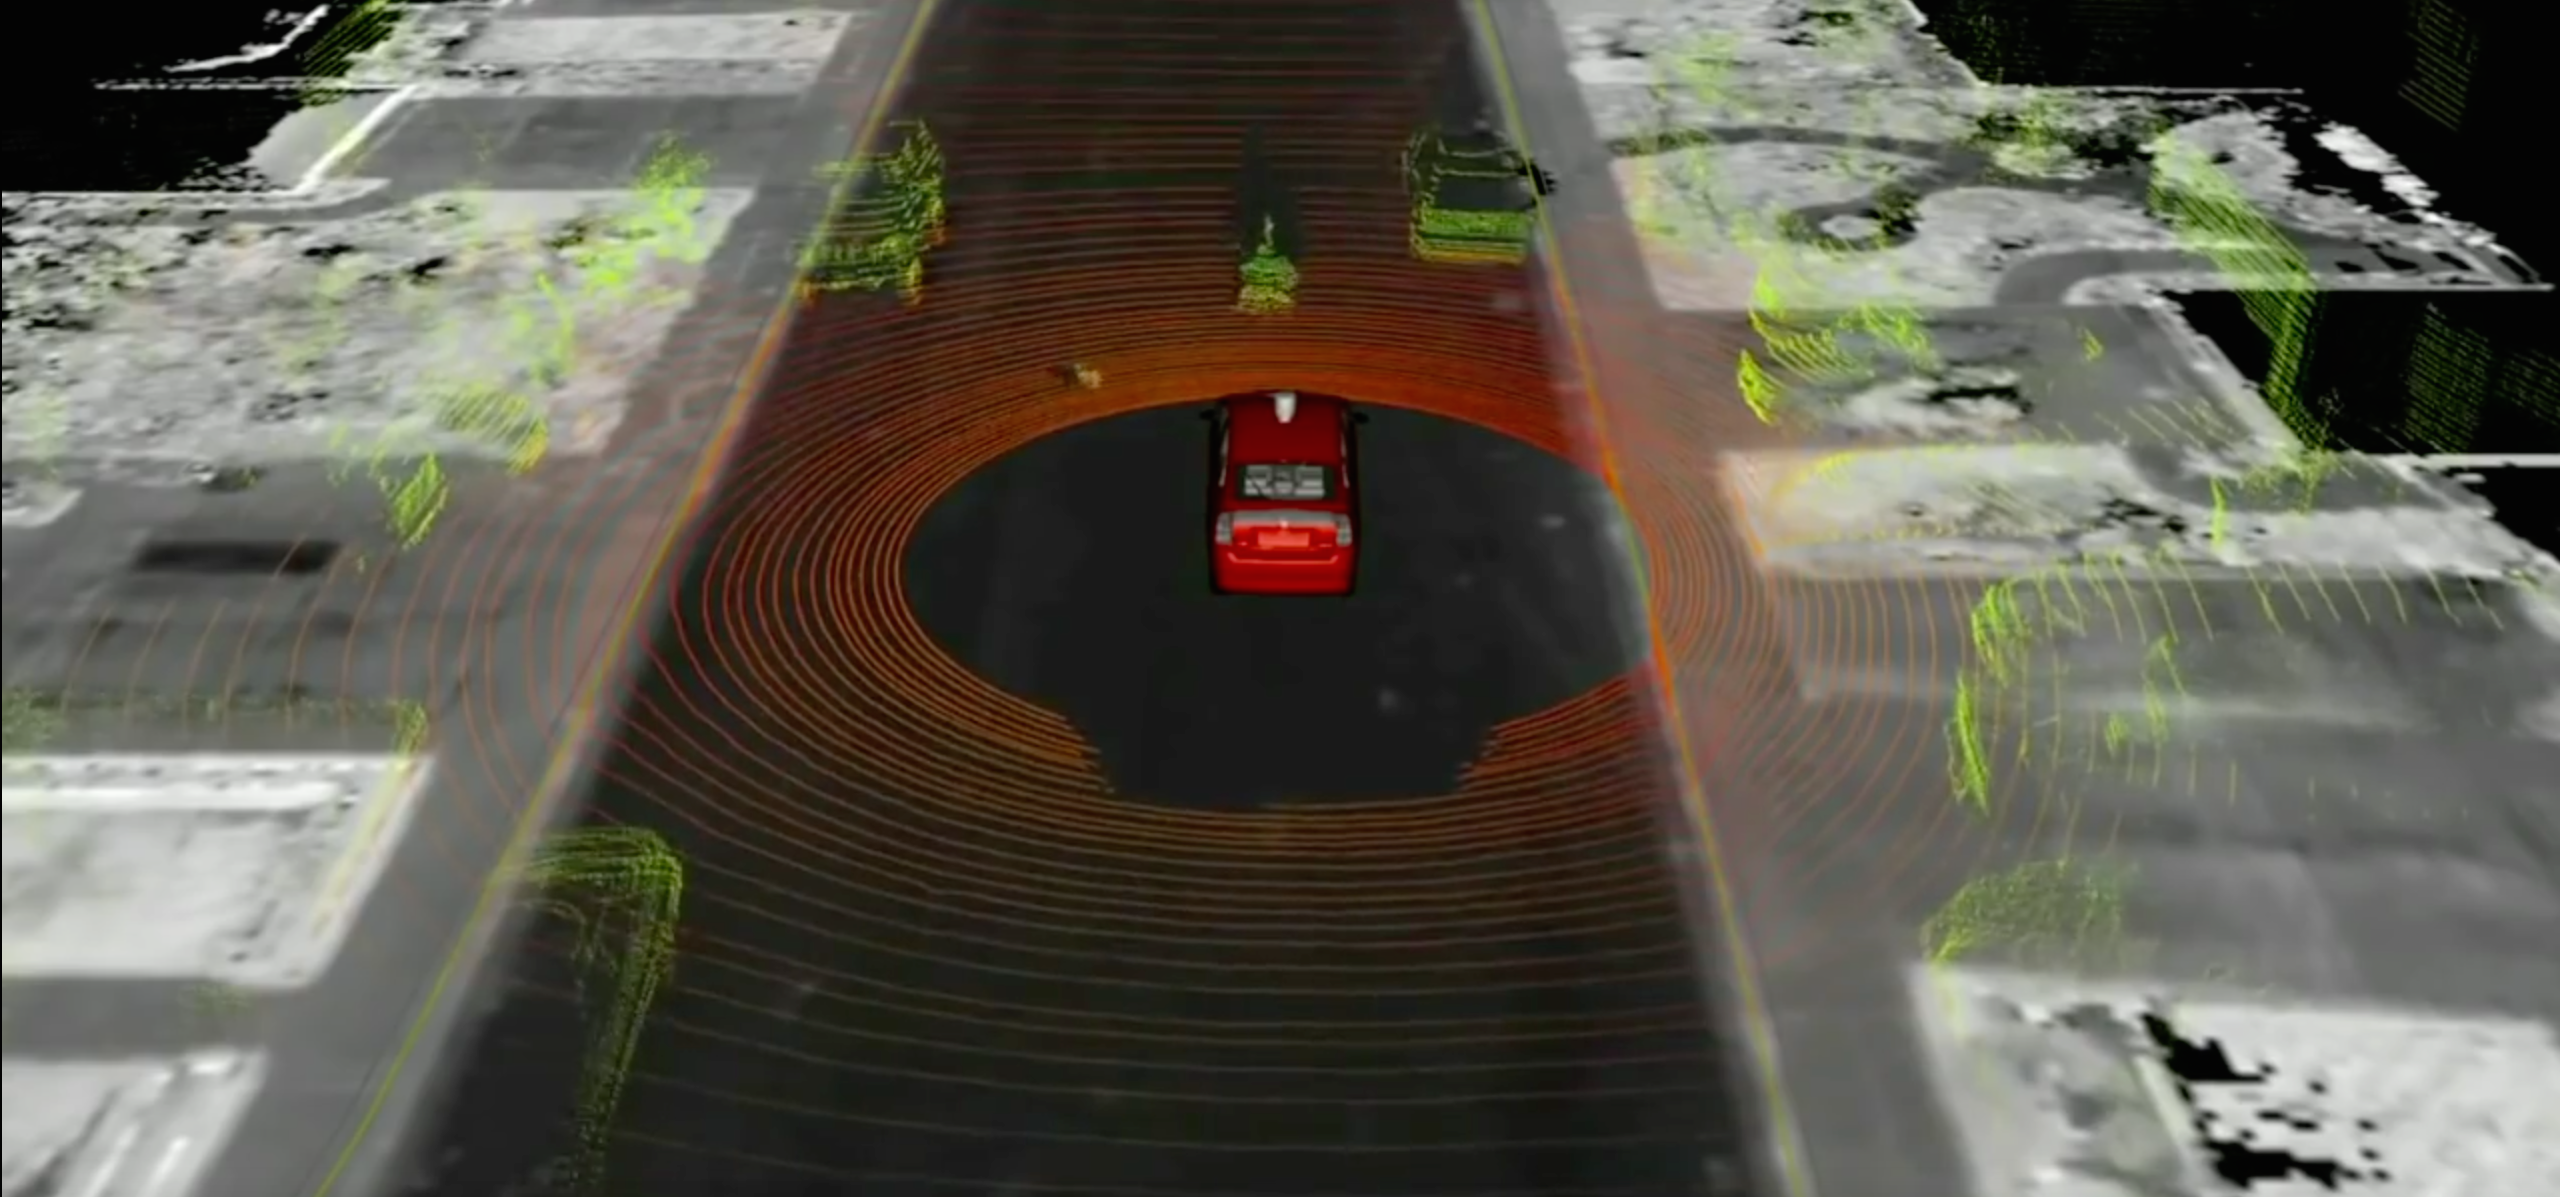
\includegraphics[width=\columnwidth]{figures/duck.png}
 	\caption{New Challenges: A woman in a wheelchair chasing a duck; autonomous vehicles are driving in real traffic engineers face an extremely long tail of events for which they must provide solutions}
 \end{figure}
 
 
 %As Brian Soublet of the California DMV pointed out, he knows how to test a 16-year-old's driving skills, but he can't say the same for a car. At the same time, these regulators know that when a death inevitably happens—no amount of %self-driving cars will reduce annual road deaths to zero—they'll be attacked for allowing unsafe vehicles on the road.
 
 
 \subsection{The APEX approach}
 The APEX tool represents a new approach to solving both the problems of the Urban Challenge and investigating rare events encountered only through on road driving and testing. Unlike other tools capable of verifying controllers for hybrid systems we require almost no abstraction. Most current approaches look at only the behavioral layer and assume perfect implementation of plans at the motion planning layer. Instead, we propose that the behavioral layer is used to generate sequences of problems to be investigated at the level of motion planning and trajectory tracking.  Thus, APEX addresses the safety verification issue by leveraging new results in hybrid systems and reachability analysis \cite{gao2013satisfiability} to convert a brute force search over real intervals (which is intractable) into a set of finite sequences of bounded reachability problems. 
 \begin{figure}
 	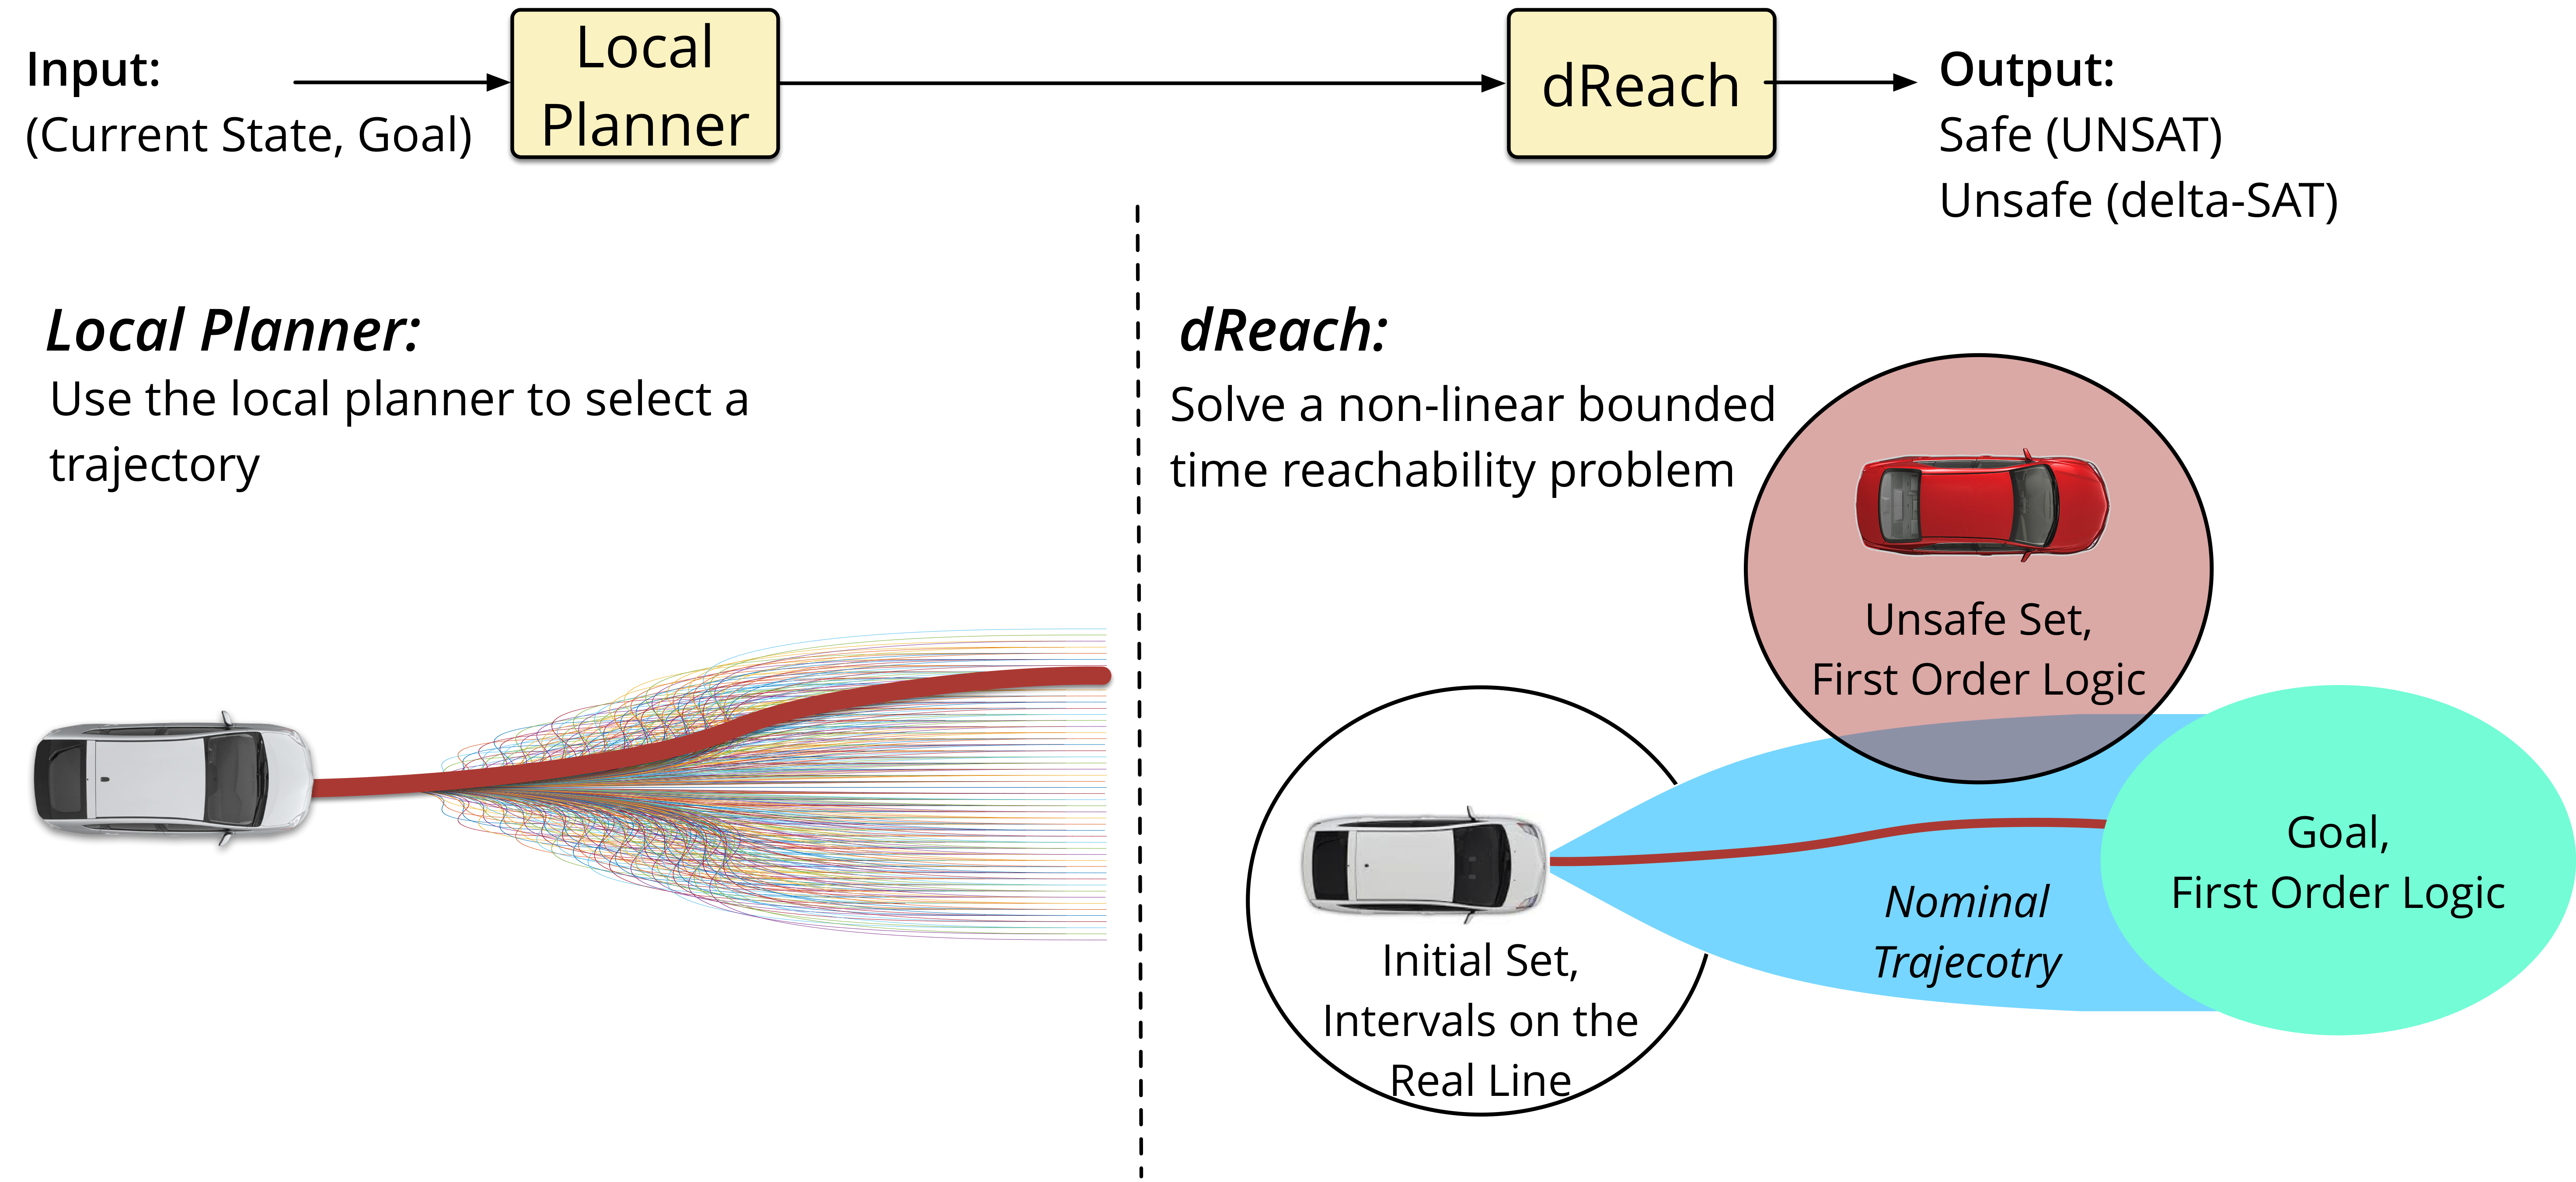
\includegraphics[width=\columnwidth]{Figures/tool_single}
 	\caption{A single offline execution of the APEX tool calls the local planner associated with the AV in order to generate a reachability problem}
 \end{figure}
 
 Using APEX we capture the output of trajectory generation and optimization based methods outside of the formal model of the system. Using such information, we generate a sequence of verification problems by running the through realistic vehicle dynamics and low level controls. The software which runs on the vehicle is used directly for verification. If a rare event is encountered and recorded by a real vehicle and a new rule or controller is added to the AV it is imperative that the manufacturer have high confidence that the modification will not induce new errors which are not evident in a single trace. APEX can make the most of rare events and scenarios; given a template we could find every possible instantiation and prove it is impossible for solution to make a decision leading to crash. The key features of our approach are:
 \begin{itemize}
 	\item Use of realistic planning software which runs on actual vehicles.
 	\item Modular vehicle model construction which can easily be replaced when new algorithms or alternate vehicle dynamics are necessary.
 	\item Non-conservative evaluation of safety at the level of the ego-vehicles actual spatial-temporal evolution. 
 \end{itemize}
 
 Thus, verification of realistic scenarios under all possible configurations over a length of 1-7 seconds is potentially feasible. Using such an approach a manufacturer, regulator, or insurer can begin to build a library of scenarios on which to test new vehicle software or updates made to the behavioral layer made through a reinforcement learner.
 
 \subsection{Contributions}
 
 Our main contribution is a design-time approach to \emph{formally} verifying the trajectory planning and trajectory tracking stacks of an ADAS/AV as they interact with potentially dynamic participants in a \emph{variety} of driving scenarios.
 This approach is implemented in a software tool, APEX, and illustrated with examples of a lane change maneuver.
 The verification approach has two characteristics:
 \vspace{-10pt}
 \begin{itemize}
 	\item It is formal: we are \emph{guaranteed} that if APEX determines a scenario to be safe, then it is safe. 
 	No amount of simulation can find an unsafe behavior in a scenario verified as correct by APEX.
 	\item It allows the use of an arbitrary trajectory planner, for example, it could be code or an abstraction. 
 	That is, there is no need to model the trajectory planner, which is often very complex software.
 	Moreover, the same trajectory planner can then be run on a real vehicle.
 	In the case study presented in this paper, APEX uses a trajectory planner that has been tested on  a real vehicle.	
 \end{itemize}
 In APEX, the verification engineer can
 \vspace{-10pt}
 \begin{itemize}
 	\item Specify the low-level dynamics of the vehicle, including the trajectory tracker. 
 	Unlike other approaches and existing tools the dynamics can be nonlinear. 
 	The default model in APEX is a 7D bicycle model.
 	\item Provide a motion planner that takes in a starting position and end position and returns a trajectory that links the two points.
 	The motion planner can be \emph{any piece of software}: there are no restrictions on it.
 	The default planner in APEX is a state lattice planner incorporated in ROS and tested on a real vehicle. Figure \ref{fig:ros} shows the planner GUI available as part of Autoware
 	\cite{kato}.
 	\item Specify a sequence of goal positions (or \emph{waypoints}) that the vehicle must visit, or a behavioral planner that computes these waypoints in a reactive manner.
 	The default behavioral planner in APEX is a simple 2-state automaton that decides whether to execute lane following or lane changing. However, we expect that designers will implement many other more complex behavioral planners.
 	\item Specify the uncertainty sets for the ego vehicle and the other agents in the scenario.
 	\item Specify the unsafe conditions to be avoided by the vehicle. 
 	APEX supports a rich specification language, Metric Interval Temporal Logic (MITL) for the description of unsafe behaviors \cite{alur91benefits}.
 \end{itemize}
 
 
 
 APEX will then verify, in an exhaustive fashion, that the ego vehicle can complete the scenario under the specified uncertainty, or return a specific case where it fails.
 The engineers can then use this \emph{counter-example} in order to debug the controllers, and better understand how to avoid this failure at design-time. 
 \begin{figure}[h]
 	\centering
 	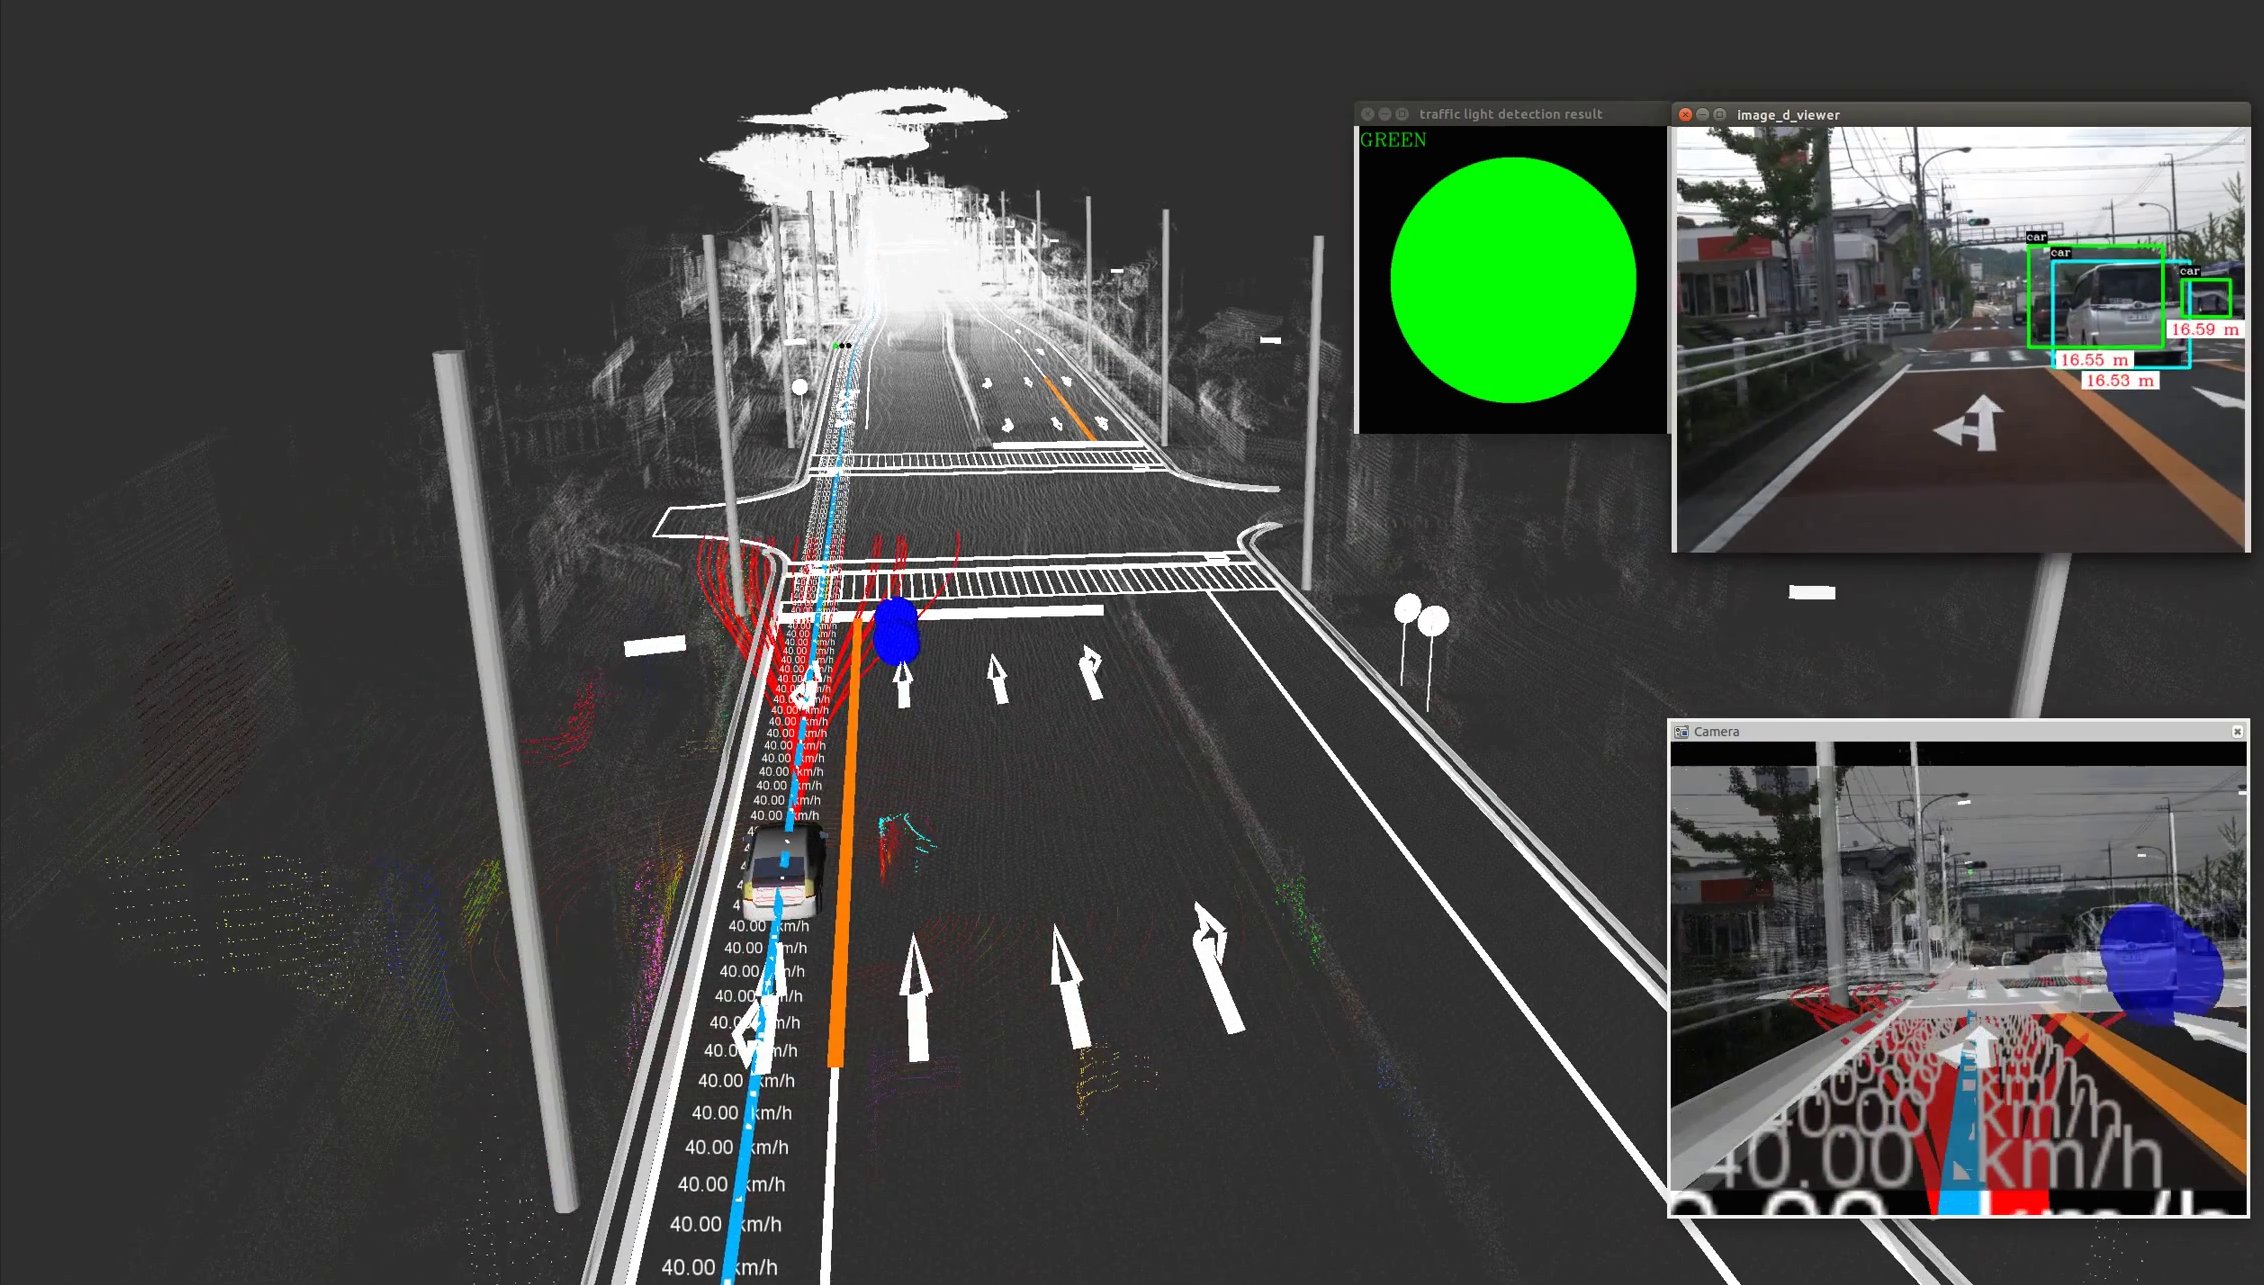
\includegraphics[width = \textwidth]{figures/apex_planning.png}
 	\vspace{-10pt}
 	\caption{ROS APEX planning implementation GUI.}
 	\vspace{-10pt}
 	\label{fig:ros}
 \end{figure}
 
 One real-world example of an AV software bug related to plan execution was highlighted by the first ever crash between AVs at the Urban Challenge \cite{fletcher2008cornell}. At the time of the accident, participants noted that there are no known \quotes{formal methods that would allow definitive statements about the completeness or correctness of a vehicle interacting with a static environment, much less a dynamic one} \cite{urmson2008autonomous}. It is beyond the scope of this paper to review the numerous developments in verification and synthesis technology;
 we note attempts exist to reason about the safety of autonomous vehicles in static environments via synthesis \cite{Wongpiromsarn2010}, but such methods cannot currently scale to realistic systems and are extremely conservative. In response the authors of \cite{Wongpiromsarn2010} propose a receding horizon framework, but still rely on coarse grid-based abstractions. Others have sought to verify Adaptive Cruise Control Algorithms (ACC) which severely restrict scenarios in which the car may operate (no lane changes) \cite{nilssoncorrect}. Finally, some research which eschews discretization in favor of continuous linearized dynamics focuses on moving the verification task online \cite{althoff2012}.
 
